\parbox{0.9\textwidth}
{
    Eine komplexe Zahl als Wertepaar kann mit einem \textbf{Vektor im Vektorraum} $\mathbb{R}^2$ verglichen werden,
    wobei auch Rechenarten, wie Addition und Multiplikation (mit reellen Zahlen) analog zur Vektoraddition und Vektormultiplikation sind.
    Der Vektorraum bei komplexen Zahlen hat wie der Vektorraum von $\mathbb{R}^2$ \textbf{zwei Koordinatenachsen}.
    Dabei gibt die \textbf{x-Achse den reellen Anteil und die y-Achse den imaginären Anteil} der komplexen Zahlen an.
    Für die Darstellung komplexer Zahlen wird die Gleichung 
    $\mathbf{z = \left(a; b\right) = a \cdot \left(1; 0\right) + b \cdot \left(0;1\right)}$ verwendet.
    Dabei ist das Wertepaar $\mathbf{\left(1; 0\right) = 1}$ als Einselement definiert, während das Wertepaar 
    $\mathbf{\left(0; 1\right) = i}$ angibt. Es ergibt sich also folgende Gleichung: 
    $\mathbf{z = a \cdot 1 + b \cdot i = a + bi}$.
}

\begin{center}
    \resizebox{9.5cm}{9.5cm}{
    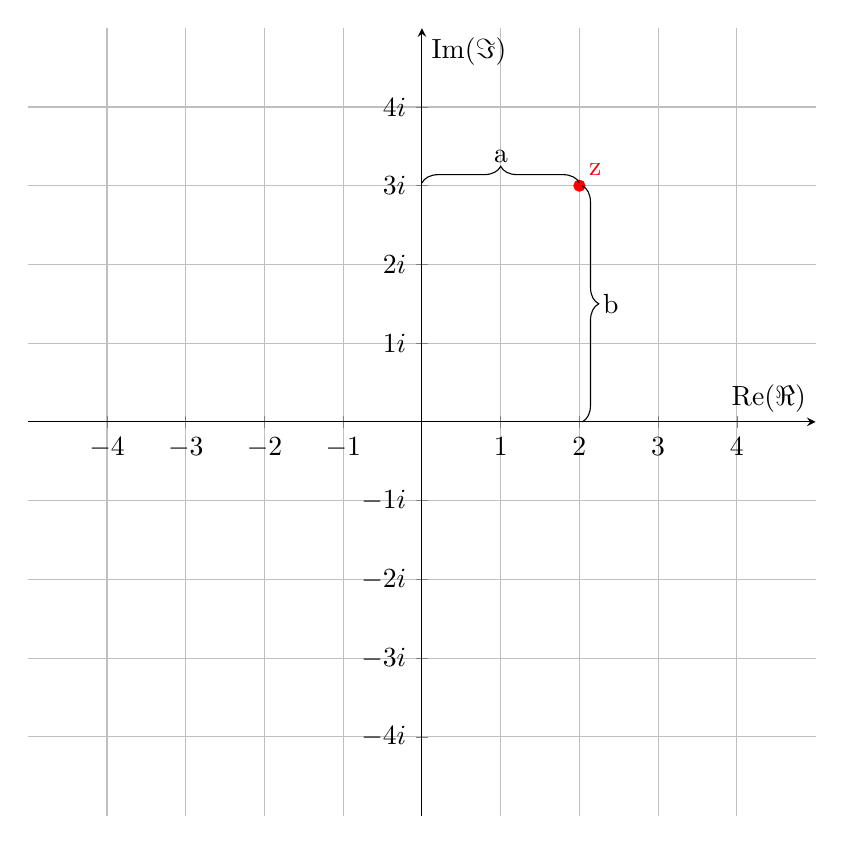
\begin{tikzpicture}
        \begin{axis}[
            samples=100,
            axis lines=center,
            x=1cm,
            y=1cm,
            xmin=-5, xmax=5,
            ymin=-5, ymax=5,
            xtick={-4, -3,...,3, 4},
            ytick={-4, -3,...,3, 4},
            xticklabels={$-4$,$-3$,$-2$,$-1$,$0$,$1$,$2$,$3$,$4$},
            yticklabels={$-4i$,$-3i$,$-2i$,$-1i$,$0i$,$1i$,$2i$,$3i$,$4i$},
            xlabel=$\mbox{Re} (\Re)$,
            ylabel=$\mbox{Im} (\Im)$,
            grid=major,
        ]

        \draw[color = red, fill] (2, 3) circle[radius=2pt, fill] node[above right]{ z };
        
        \draw[decorate, decoration = {brace,amplitude=6pt,raise=1pt}] (0, 3) -- (2, 3) node[midway, above, yshift=5pt]{a};
        \draw[decorate, decoration = {brace,amplitude=6pt,raise=1pt,mirror}] (2, 0) -- (2, 3) node[midway, right, xshift=5pt]{b};

        \end{axis}
    \end{tikzpicture}
}
\end{center}

